\documentclass[5p]{elsarticle}

\usepackage{lineno,hyperref}
\usepackage{amsfonts}
\usepackage{amsmath}
\usepackage{mathtools}

\modulolinenumbers[5]

\journal{Journal of \LaTeX\ Templates}

%%%%%%%%%%%%%%%%%%%%%%%
%% Elsevier bibliography styles
%%%%%%%%%%%%%%%%%%%%%%%
%% To change the style, put a % in front of the second line of the current style and
%% remove the % from the second line of the style you would like to use.
%%%%%%%%%%%%%%%%%%%%%%%

%% Numbered
%\bibliographystyle{model1-num-names}

%% Numbered without titles
%\bibliographystyle{model1a-num-names}

%% Harvard
%\bibliographystyle{model2-names.bst}\biboptions{authoryear}

%% Vancouver numbered
%\usepackage{numcompress}\bibliographystyle{model3-num-names}

%% Vancouver name/year
%\usepackage{numcompress}\bibliographystyle{model4-names}\biboptions{authoryear}

%% APA style
%\bibliographystyle{model5-names}\biboptions{authoryear}

%% AMA style
%\usepackage{numcompress}\bibliographystyle{model6-num-names}

%% `Elsevier LaTeX' style
\bibliographystyle{elsarticle-num}
%%%%%%%%%%%%%%%%%%%%%%%



\begin{document}

\begin{frontmatter}

\title{Obscured by the Cloud: A resource allocation framework to model Cloud outage events\tnoteref{mytitlenote}}
%%\tnotetext[mytitlenote]{}

%% Group authors per affiliation:
%% \author{Elsevier\fnref{myfootnote}}
%% \address{Radarweg 29, Amsterdam}
%% \fntext[myfootnote]{Since 1880.}

%% or include affiliations in footnotes:
\author[mymainaddress]{Jonathan Dunne\corref{mycorrespondingauthor}}
\cortext[mycorrespondingauthor]{Corresponding author}
\ead{jonathan.dunne.2015@mumail.ie}

\author[mymainaddress]{David Malone}
%%\ead[url]{www.elsevier.com}

\address[mymainaddress]{Hamilton Institute, Maynooth University, Kildare, Ireland}

\begin{abstract}
As Small Medium Enterprises (SMEs) adopt Cloud technologies and rapid delivery models to provide high value customer offerings, there is a clear focus on uptime. Cloud outages represent a challenge to SMEs and micro teams to maintain a services platform. If a Cloud platform suffers from downtime this can have a negative effect on business revenue. Additionally outages can divert resources from product development/delivery tasks to reactive remediation. These challenges are more immediate for SMEs or micro teams with a small pool of resources at their disposal. In this paper we present a framework that can be used to model the arrival of Cloud outage events. Such a framework can be used by Cloud operations teams to manage their scarce pool of resources to resolve outages, thereby minimising impact to service delivery. We conducted analysis of over three 300 Cloud outage events from an enterprise data set. We modelled the inter arrival and service times of each outage event and found a Pareto and lognormal distribution to be a suitable fit. We used this result to produce a special case of the G/G/1 queue system to predict the busy times of DevOps personnel. We also investigated dependence between overlapping outage events. Our busy time predictive queuing model compared favourably with observed data, 72\% precision was achieved using one million simulations. 

\end{abstract}

\begin{keyword}
Outage simulation \sep Resource allocation model \sep Queuing Theory \sep Cloud computing
\end{keyword}

\end{frontmatter}

\linenumbers

\section{Introduction}
Cloud outage prediction and resolution is an important activity in the management of a Cloud service. Recent media reports have documented cases of Cloud outages from high profile Cloud service providers \cite{CRN2016outage}. During 2016 alone the CRN website has documented the ten highest profile Cloud outages to have occurred so far.  Due to the increasing complex nature of the data centre infrastructure, coupled with the rapid continuous delivery of incremental software updates, it seems that Cloud outages are with us for the time being.

% Added references for monitoring solutions

For operations teams that maintain a Cloud infrastructure, they rely on state of the art monitoring and alert systems to determine when an outage occurs. Examples of monitoring solutions include: New Relic \cite{newrelic}, IBM Predictive Insights \cite{predinsight} and Ruxit \cite{ruxit}. Once a new outage is observed, depending on the outage type (e.g. Software component, infrastructure, hardware etc), additional relevant experts may be called to remediate the issue. The time taken to resolve the issue may depend on a number of factors: ability to find the relevant expert, swift problem diagnosis and velocity of pushing a fix to production systems. 

Both SME's and micro teams within large organisation's face a number of challenges when adopting a Cloud platform and a mechanism to deliver products and services. A number of recent studies have outlined that both frequency and duration of outage events are key challenges \cite{InfoWorld2015outage}. Almost all European SME's (93\%) employ less than ten people \cite{europa2015sme}. Ensuring that adequate skills and resources are available to accommodate incoming outage events is highly desirable.

In this paper we propose a framework that a micro team or SME's can leverage to best manage their existing resource pool. 

The core idea of this framework is for operations teams to use a special case of the G/G/1 queue to model the inter-arrival and service times of outage events. This article consists of a study of outage event data from a large enterprise dataset. By modelling both inter-arrival and service outage times, a special case of the G/G/1 queue is developed. This G/G/1 queue is then tested against an off the shelf queue model (M/M/1) to compare and contrast queue busy time prediction. Finally our framework also considers dependence between overlapping outage events. 

To help researchers reproduce and extend this study, pseudo-code of the queue modelling framework is provided. By utilising this queue framework, researches will have the ability to test their preferred case of the G/G/1 model against the M/M/1 model.

% Moved the justification for Queuing over Renewal Reward systems to here

It should be noted that the area of it should be noted that the branch of probability theory called: Renewal Reward Process \cite{blackwell1948renewal}\cite{jewell1967simple} was also considered as part of this study. In fact on closer inspection the processes are quite similar.  For example the time between successive outages on a Cloud system could be assigned as the holding times, the rewards may be seen as the repair costs (service times) for each outage event. However a key application of this study is to understand whether a queue model could be used to simulate outage arrivals. If an effective simulation model can be found, can we use this model to aid resource planning of personnel within a micro team or SME.

By looking at the traffic intensity and the queue length we can determine how resources need to be deployed with a micro team or SME. The applications of a Renewal Reward process relate more to understanding of: the age of a software component, the remaining lifetime of a software component, and the replacement reward/penalty of a software component. These questions are all valid, we discuss these applications briefly in our conclusion.

Downtime is bad for business. Whether a company provides a hosting platform, more commonly known as Platform as a Service (PaaS), or for a company that consumes such a platform to deliver their own services, more commonly known as Software as a Service (SaaS). The end result is the same: Business disruption, lost revenue and recovery/remediation costs. A recent US study  looked at the cost of data centre downtimes and calculated the mean cost to be \$5617 per minute of downtime \cite{DCcost}.

In the current literature a framework to model Cloud outage events is absent. This study observed that outage events arrive over a period of time, which require fixing to return a system to a steady state. With these attributes in mind, our literature search focuses on queuing theory and distribution fitting for repairable systems.

Another consideration is the idea of event dependence. Typical off the shelf single-server queue models such as M/M/1 and G/G/1 assume that the inter-arrival and service times between events are independent \cite{MM1}. However if some form of dependence is found between events how useful would a queuing model which assumes independence compare against that of a queuing model with dependence properties.

% Research Questions here

This study aims to answer a number of questions. First, how are the inter-arrival times of Cloud outage events distributed? Second, How are the service times of Cloud outage events distributed?  Third, How can an effective queuing model be built to simulate outage event traffic? Fourth, How are inter-arrival and service times correlated? Fifth, are overlapping outage events related or can we treat each event as independent? 

% Research Questions above

% Additional UK and EU studies added in this paragraph

Further motivation is driven by recent reports and studies into the adoption of Cloud computing.  Carcary et al. \cite{carcary2014adoption}, Alshamaila et al.  \cite{alshamaila2013cloud} and Oliveira et al. \cite{oliveira2014assessing} all conducted studies on Cloud computing adoption by SMEs. The general consensus is that, there is no single factor which impedes Cloud adoption. The main constraints noted were: Security/compliance/data protection along with geo-restriction and compatibility to legacy systems. It was also noted that manufacturing and services sectors have different concerns in relation to Cloud computing adoption. Which indicates some level of customisation is required to meet the needs across different industries. Additionally Gholami et al. \cite{gholami2016Cloud} provided a detailed review of current Cloud migration processes. One of the main migration concerns mentioned was the unpredictability of a Cloud environment. Factors that led to this unpredictability included: Network outages and middleware failures. The study concluded that a fixed migration approach is not possible to cover all migration scenarios due to architecture heterogeneity.

The rest of this article is divided up into the following sections: Section 2 introduces background and related work. Section 3 discusses the data set collected (and associated study terminology), outlines the questions that are answered by this study and the limitations of the dataset. Section 4 outlines the experimental approach and associated results. Section 5 discusses the results of our experiments. Finally in Section 6, we conclude this paper and discuss future work.

\section{Background and related work}

The following section provides some background information on two common Cloud services: SaaS and PaaS. We then review high profile Cloud outages that have made the media headlines. Finally this section concludes with a in-depth look at relevant studies in the field of repairable systems modelling, queuing theory and Cloud outage studies.

\subsection{Software as a Service}
SaaS is defined as a delivery and licensing model in which software is used on a subscription basis (e.g. monthly, quarterly or yearly) and where applications or services are hosted centrally \cite{Cloudbook2015}. The key benefits for software vendors are the ability for software to be available on a continuous basis (on-demand) and for a single deployment pattern to be used. It is this single deployment pattern that can greatly reduce code validation times in pre-release testing, due to the homogeneous architecture. Central hosting also allows for rapid release of new features and updates through automated delivery processes \cite{datacentre2015}. 

SaaS is now ubiquitous, while initially adopted by large software vendors (e.g. Amazon, Microsoft, IBM, Google and Salesforce) many micro teams SMEs are now using the Cloud as their delivery platform and licensing model of choice \cite{CRN2015providers}. 

\subsection{Platform as a Service}
PaaS is defined as a delivery and platform management model. This model allows customers to develop and maintain Cloud based software and services without the need for building and managing a complex Cloud based infrastructure.

The main attraction of PaaS is that it allows SME's to rapidly develop and deliver Cloud based software and services. While focusing on their core products and services SME's are less distracted by having to design, build and service a large complex Cloud based infrastructure. 

However one drawback of PaaS is that an SME may not have a full view of the wider infrastructure. Therefore if an outage event occurs at an infrastructure level (e.g. Network, Loadbalancer) an SME may be unaware of the problem until the problem is reported by a customer.

Many companies now offer PaaS as their core service. Once seen as the preserve of a large organisation (e.g. Amazon EC2, Google Apps and IBM Bluemix) a number of smaller dedicated companies also offer PaaS (e.g. Dokku, OpenShift and Kubernetes) \cite{Paas2016}.


\subsection{High profile Cloud outages}
A Cloud outage is the amount of time that a service is unavailable to the customer. While the benefits of Cloud systems are well known, a key disadvantage is that when a Cloud environment becomes unavailable it can take a significant amount of time to diagnose and resolve the problem. During this time the platform can be unavailable for customers.

One of the first Cloud outages to make the headlines was the Amazon outage in April 2011. In summary, the Amazon Cloud experienced an outage that lasted 47 hours, the root cause of the issue was a configuration change made as part of a network upgrade. While this issue would be damaging enough for Amazon alone, a number of consumers of Amazon's Cloud platform (Reddit, Foresquare) were also affected. \cite{InfoWorld2015outage} 

Dropbox experienced two widespread outages during 2013 \cite{Talbot013DBoutage, Etherington2013DBoutage}. The first in January, users were unable to connect to the service. It took Dropbox 15 hours to restore a full service. No official explanation as to the nature of the outage was given. The second occurred in May, again users were unable to connect to the service. This outage lasted a mere 90 minutes. Again no official explanation was provided.

Table I provides a summary of highest profile Cloud outages observed so far this year (up to June 2016)\cite{CRN2016outage} . While great improvements have been made in relation to redundancy, disaster recovery and ring fencing of critical services, the big players in Cloud computing are not immune to outages.

\begin {table*}[]
\caption {Summary of high profile Cloud outages in the first half of 2016} 
\begin{flushleft}

\begin{tabular}{l | l | l | p{11.4cm} l} \bf {Company} & \bf {Duration} & \bf {Date} & \bf {Outage Details}  
\\ \hline Office 365 & Several days &  18th Jan & Users reported issues accessing their Cloud based mail services. The defect was identified and a software fix was applied. This fix proved unsuccessful, thereafter  a secondary fix was developed and applied which was successful.
\\ \hline Twitter & 8 hours  & 19th Jan & Users experienced general operational problems after an internal software update was applied to the production system with faulty code. It took Twitter 8 hours to debug and remediate the defective code.
\\  \hline Salesforce & 10 hours  &  3rd March &  European Salesforce users had their services disrupted due to a storage problem in their EU Data Centre. After the storage issue was resolved, users reported performance degradation.
\\  \hline Symantec & 24 Hours  &  11th April &  A portal to allow customers to manage their Cloud  security services became unavailable. The exact nature of the outage was undisclosed. Symantec were required to restore and configure a database to bring the system back online.
\\ \hline Amazon & 10 hours  & 4th June & Local storms in Australia caused Amazon Web Services to lose power. This resulted in a number of EC2 instances to fail, which affected both SaaS and PaaS customers. 
\\ \hline 

 \end{tabular}
\end{flushleft}
\end{table*}

% Modified the name of the section 2.4
\subsection{Cloud outage and software reliability studies}
A number of studies have been conducted in relation to Cloud outages. Additionally, research has been carried on the time observed to service problems in repairable systems.  A summary of these studies are discussed below. \par

Yuan et al. \cite{yuan2014simple} performed a comprehensive study of distributed system failures. Their study found that almost all failures could be reproduced on reduced node architecture and that performing tests on error handling code could have prevented the majority of failures. They conclude by discussing the efficacy of their own static code checker as a way to check error-handling routines. \par

Hagen et al. \cite{hagen2012efficient} conducted a study into the root cause of the Amazon Cloud outage on April 21st 2011. Their study concluded that a configuration change was made to route traffic from one router to another, while a network upgrade was conducted. The backup router did not have sufficient capacity to handle the required load. They developed a verification technique to detect change conflicts and safety constraints, within a network infrastructure prior to execution. \par

Li et al \cite{li2013Cloud} conducted a systematic survey of public Cloud outage events. Their findings generated a  framework, which classified outage root causes. Of the 78 outage events surveyed they found that the most common causes for outages included: System issues i.e. (human error, contention) and power outages being the primary root cause. \par

Sedaghat et al \cite{sedaghat2015hard} modelled correlated failures caused by both network and power failures. As part of the study the authors developed a reliability model and an approximation technique for assessing a services reliability in the presence of correlated failures. \par 

Potharaju and Navendu \cite{potharaju2013network} conducted a similar study in relation to network outages, with focus on categorising intra and inter data centre network failures. Two key findings include: Network redundancy is most effective at inter-datacentre level and interface errors, hardware failures and unexpected reboots dominate root cause determination. \par

Bodik et al \cite{bodik2012surviving} analysed the network communication of a large-scale web application. Then proposed a framework that achieves a high fault tolerance with reduced bandwidth usage in outage conditions. \par 

Synder et al \cite{snyder2015evaluation} conducted a study on the reliability of Cloud based systems.The authors developed an algorithm based on a non-sequential Monte Carlo Simulation to evaluate the reliability of large scale Cloud systems. The authors found that by intelligently allocating the correct types of virtual machine instances, overall Cloud reliability can be maintained with a high degree of precision. \par

Kenney \cite{kenny1993estimating} proposes a model to estimate the arrival of field defects based on the number of software defects found during in-house testing. The model is based on the Weibull distribution which arises from the assumption that field usage of commercial software increases as a power function of time. If we think of Cloud outages as a form of field defect, there is much to consider in this model. For example, the arrival of Cloud outages in the the field could be modelled with a power law distribution (e.g. Pareto distribution) as a starting point. \par 

Kleyner and O'Connor \cite{o2011practical} propose an important thesis regarding reliability engineering. While emphasis is placed on measuring reliability for both mechanical and electrical/electronic systems, the authors do broaden their scope to discuss reliability of computer software. One aspect of interest is their discussion of the lognormal distribution and its application in modelling for system reliability with wear out characteristics and for modelling the repair times of maintained systems. \par

Almog \cite{almog1979study} analysed repair data from twenty maintainable electronic systems to validate whether either the lognormal or exponential distribution would be a suitable candidate distribution to model repair times. His results showed that in 67\% of datasets the lognormal distribution was a suitable fit, while the exponential was unsuitable in 62\% all of datasets. \par

Adedigba \cite{adedigba2005statistical} analysed the service times from a help desk call centre. Her study showed that the exponential distribution did not provide a reasonable fit for call centre service times. However a log-normal distribution was a reasonable fit for overall service times. Her study also showed that a phase-type distribution with three phases provided a reasonable fit for service times for specific jobs within the call centre job queue. \par

% Added a new reference based on feedback from reviewer #2
Alsoghayer and Djemame \cite {alsoghayer2014resource} propose a mathematical model to predict the risk of failures with Grid and Cloud based infrastructures. The model uses the observed mean time to failure and the mean to repair for prediction. The authors found the best model to predict the time between failures is a Weibull distribution, while the repair (service) times as best modelled by a lognormal distribution.

% Modified this paragraph as per Review #1's comments
As can be seen from the literature review a number of studies have been conducted into Cloud outage failures and the inter-arrival / repair times of computer systems. However there are no studies that conduct end to end research of outage events to build a queue model to predict the likely busy time and resource management of DevOps teams. Our proposed queue model aims to plug the gap that has been identified in the current literature.

\section{Data set and research methodology}

Cloud outage studies have been shown to provide an effective way to highlight common failure patterns \cite{InfoWorld2015outage}. In this and subsequent sections our study will present a data set and queuing model. The aim of which is to illustrate its efficacy in modelling Cloud outage events. 

% added a comment on what resources were modelled.
Our dataset is taken from an enterprise cloud system which details all outage events over an eighteen month period. In each case we had access to the full outage report log. For each outage, we observed the arrival time of each event and how long each outage took to repair. With each arrival time known the inter-arrival time between each outage was computed. We used the repair time duration as the service time.

A number of points related to the dataset are summarised in Table 2. 

\begin {table*}[]
\caption {Summary of dataset metrics} 
\begin{center}
\begin{tabular}{p{4cm} |  p{11cm}} \hline \bf{Metric} & \bf{Value}
\\ \hline Number of outage events & 331 
\\ Data collection duration & 18 months (January 2015 to June 2016) 
\\ Software components & Business Support System (BSS), Collaboration, E-mail, and Social  	
\\ Number of Data Centres & 3 
\\ Programming Language & Java 
\\ Operating System & Linux 
\\ Hardware & Intel based. (Mixture of physical and virtual systems)
\\ Load Balancing & F5
\\ \hline
\end{tabular}
\end{center}
\end{table*}

% added an extra paragraph to justify the metrics shown
It is important to affirm the Programming Language, OS, Hardware and Load Balancing solution used as part of the Enterprise solution. These metrics may be underlying factors in the root cause of the observed outages. Further investigation into the root cause of each is beyond the scope of this article. We discuss this matter in our Study limitations subsection below.

Product development follows a Continuous delivery (CD) model whereby small amounts of functionality are released to the public on a monthly basis. This study focuses on the following aspects of the outage event data: The inter-arrival time between each outage, the time to service each outage event and whether or not overlapping outage events are related.

% Added DevOps books as reference points
The following terminology will now be defined to provide clear context. These majority of these definitions are referenced from a number of sources such as ``What is DevOps?'' by Mike Loukides \cite{loukides2012devops} and ``The Phoenix Project'' by Kim et al. \cite{kim2014phoenix}.

\begin{description}
 \item [Downtime (Outage)] The term downtime is used to refer to periods when a system is unavailable. Downtime or outage duration refers to a period of time that a system fails to provide or perform its primary function. 
 \item  [Micro Team] In information technology a micro team is typically staffed by three to five persons. Each person within the group has a specific role; Developer, Test Engineer, Automation specialist and a people manager. With each skill set clearly defined there is little to no overlap in terms of role definition. Each role within the team can be considered a single point of failure.
  \item [Tiger Team] A tiger team is a group of experts assigned to investigate and/or solve technical or systemic problems. 
 \item [DevOps] Is a practice that highlights the collaboration between software development and infrastructure personnel. DevOps may also refer to a team which has a core function to build, deploy and maintain a Cloud infrastructure. 
% Added Queuing theory books as reference points
 \item [Queuing theory] Is the study of events that form waiting lines or queues. In queuing theory, a model is constructed so that queue lengths, inter-arrival and service times can be predicted \cite{kleinrock1975queuing, gross2008fundamentals, sundarapandian2009probability}.
\end{description}

Prior to outlining our research questions, it is useful to understand why queuing theory could be used to model Cloud outages events. Outages begin at a specific point in time. The problem is then diagnosed and serviced by tiger and DevOps teams. These characteristics are very similar to the properties of a queue system (i.e. inter-arrival times, service times and queue length). 

Both micro teams and SME's have less than ten employees \cite{eusmereport2015}, yet are adopting the Cloud as a method to deliver software and services. Given the unpredictability of Cloud infrastructure architecture, this study is required to understand whether a micro team / SME has adequate resources to manage future Cloud outage events. 

This study aims to answer a number of questions. First, how are the inter-arrival times of Cloud outage events distributed? Second, How are the service times of Cloud outage events distributed?  Third, How can an effective queuing model be built to simulate outage event traffic? Fourth, How are inter-arrival and service times correlated? Fifth, are overlapping outage events related or can we treat each event as independent? 

\subsection{Inter-arrival time distribution}

Probability distributions are used in statistics to infer how likely it is for an event to happen. In the case of Cloud outage inter-arrival times,  we can analyse the data and determine which distribution is the best fit. The properties of a distribution can then be used to infer the likelihood of an event happening. For distribution fitting, we used the R package fitdistrplus \cite{fitdistrplus} to fit various distributions to our dataset. To validate the efficacy of each distribution,  the authors used the R package ADGofTest \cite{ADGoF}. 

\subsection{Service time distribution}

This study has similar motivations for Cloud outage service times. Being able to determine a probability distribution that best fits this outage event dataset is a useful exercise. By combining both inter-arrival and service time distributions a queue system can then be built. This queue system can be used to model the arrival and service times of Cloud outage events. The approach to distribution fitting and validation, is the same as described in the previous sub-section. 

\subsection{Correlation between inter-arrival and service times}

Statistical correlation is used to measure how two variables are related. For this study we want to check if there is a relationship between the duration of inter-arrival and service times and if so what is the level of this relationship. 

There are a number of tests that can be conducted to determine correlation. We shall discuss these briefly.

Pearson \cite{fisher1915frequency} and Spearman's \cite{spearman1904proof} ranked coefficient use a single measure to determine the relationship between two variables. The strength of the relationship is measured between 0 (no correlation) to 1 (high correlation). Additionally the coefficient can be positive or negative indicating the type of relationship. Pearson's test is typically used when dealing with a variables with a linear relationship while Spearman's test can be used where a relationship is monotonic (whether linear or not). 

Linear regression \cite{galton1890kinship} is a method to model the relationship between two variables where one variable is dependent and the other is an  independent variable. A hypothesis test is conducted and a p-value is computed. Dependent on the size of the p-value the hypothesis of a relationship / no relationship can be accepted or rejected.

Finally autocorrelation \cite{box1970distribution} is the correlation of a variable with itself (and potentially other variables) at different points over a given time period. The test looks at the time lag between events to infer if a repeating pattern (seasonality) exists. Examining the lags of variables can be useful to determine if there are distinct cyclical patterns between variables or if these patterns are simply white noise.

For our correlation assessment we used the following functions found in the base R package: cor.test \cite{PearSpearR}, lm \cite{lmR} acf \cite{acfR} to test the relationship between inter-arrival and service times.

Correlation tests can also be used to determine dependence between variables, however we shall discuss a specific aspect of dependence in section 3.5. 

\subsection{Outage event modelling framework}

Queuing models have been used previously across many sciences to simulate the arrival and service times for a collection of events. Typically observed inter-arrival and service times data is used to derive a suitable fitting distribution. Thereafter the distribution parameters (i.e. mean, rate, shape, scale etc) are used to simulate queue traffic. Simulations allow large experiments to be undertaken which could not be conducted with the real system, and to make predictions of future behaviour.

For this study we look at how a queuing system can be used to model Cloud outage events. Our queue system was developed using the C programming language. Our study conducted 1M simulations against a G/G/1 system based on fitted sample distributions. Furthermore our study also conducted the same number of simulations against an M/M/1 queue. For the mean inter-arrival and service times we used the computed means from our Pareto and lognormal distributions.

An assessment of the usefulness of such simulations is given within the context of resource management within a micro team or SME. Can such simulations provide a reasonable degree of precision to aid resource planning of DevOps / Tiger teams with constrained levels of staffing?

\subsection{Assessment for no association and linkage between overlapping outage events}

As discussed earlier, the M/M/1 queuing system assumes that arrivals are independent. This is due to the understanding that both arrival and service times are governed by a Poisson process. For G/G/1 (i.e.general distribution) queues, we still have the same assumption of independence. However, the occurrence of cascading (i.e. dependent) outages events can play a role in the shape of both inter-arrival and service distributions. Therefore for the final part of our statistical analysis, this study formally tests whether the arrival times of overlapping outage events are independent or not. 

The following method will be used: Defect outage reports will be analysed to determine if an arrival overlaps with the service time of a prior outage event. Next the outage reports will be examined to determine if the two overlapping outages are related by component area and root cause. The outage counts will then be arranged in a 2 by 2 contingency table format. Fishers exact test for independence\cite{fisher1922interpretation}\cite{fisher1925statistical} is then conducted. For the actual test the authors used the R library fisher.test \cite{FisherExact}. 

\subsection{Study limitations / Threats to validity}

The dataset has a number of practical limitations, which are now discussed. The event data collected for this study comprised of outage reports from an enterprise system deployed over three data centres. For the purposes of event modelling the authors have assumed a simple queue. In other words a queuing system with one \lq\lq server\rq\rq. Given the lack of studies in the area of modelling Cloud outage events within a queuing framework, the authors wanted to validate such a framework in the context of a simple queue initially. 

% Section on how we could extend to multiple queue systems.
Bearing in mind that an outage of a specific type (i.e. Hardware, Network, High Availability) will typically affect a single data centre at a time, there is a class of outage (i.e. Software, Configuration) which may effect multiple systems concurrently and in parallel. Our queue model could be extended to a queue with multiple servers using the following approach. The inter-arrival and service times could each data centre could be modelled separately. Using this result we could obtain a per data centre queue busy time. For outages which affect multiple data centres we can model these events isolation to determine the probability of such an event occurring with an overlapping single data centre outage event.

For the M/M/1 simulation, in the absence of a suitably good fitting mean parameter we used the means from our inter-arrival and service time distributions.

The outage events that form part of this study are from an enterprise Cloud system. We recognise that the outage events observed, can have a variety of root causes (i.e. Configuration-Manual, Concurrency-Contention, Hardware, High availability and Network). A number of Concurrency-Contention outage events may be tied to the code base which is specific to this Cloud system. However concurrency and contention issues can occur in distributed computing systems irrespective of the underlying software code.

% Added additional justification on the use of Java
The hardware used in the Cloud environment is Intel based (i.e. x86\_64), therefore any hardware failures will be applicable to this hardware form factor, that said this a common hardware type. Additionally the programming language used to code the software services is Java. Any outage events that are related to a software defect should be compared to similar Cloud outage data where Java is used.

The outage events are applicable to the software domain of BSS, Collaboration, Email and social applications. As a consequence the analysis may not be relevant outside of this realm.

\section{Results}
The results of the study are now discussed. This section shall follow the same format as the methodology section.

\subsection{Inter-arrival time distribution}

\begin {table}
\caption {Inter-arrival time distributions :  Goodness of fit summary} 
\begin{center}
\begin{tabular}{p{2.1cm} |  p{3.1cm} | p{1.3cm}} \hline \bf{Distribution} & \bf{AD Test Statistic} & \bf{p-value}
\\ \hline Pareto & 0.53 & 0.72 
\\ loglogistic & 1.93 & 0.10
\\ lognormal & 3.79 & 0.01
\\ gamma & 632.89 & 1.83e-06	
\\ exponential & Infinity  & 1.83e-06
\\ logistic & Infinity & 1.83e-06	
\\ weibull  & Infinity & 1.83e-06 
\\ \hline
\end{tabular}
\end{center}
\end{table}

\begin{figure*}[]
\begin{center}
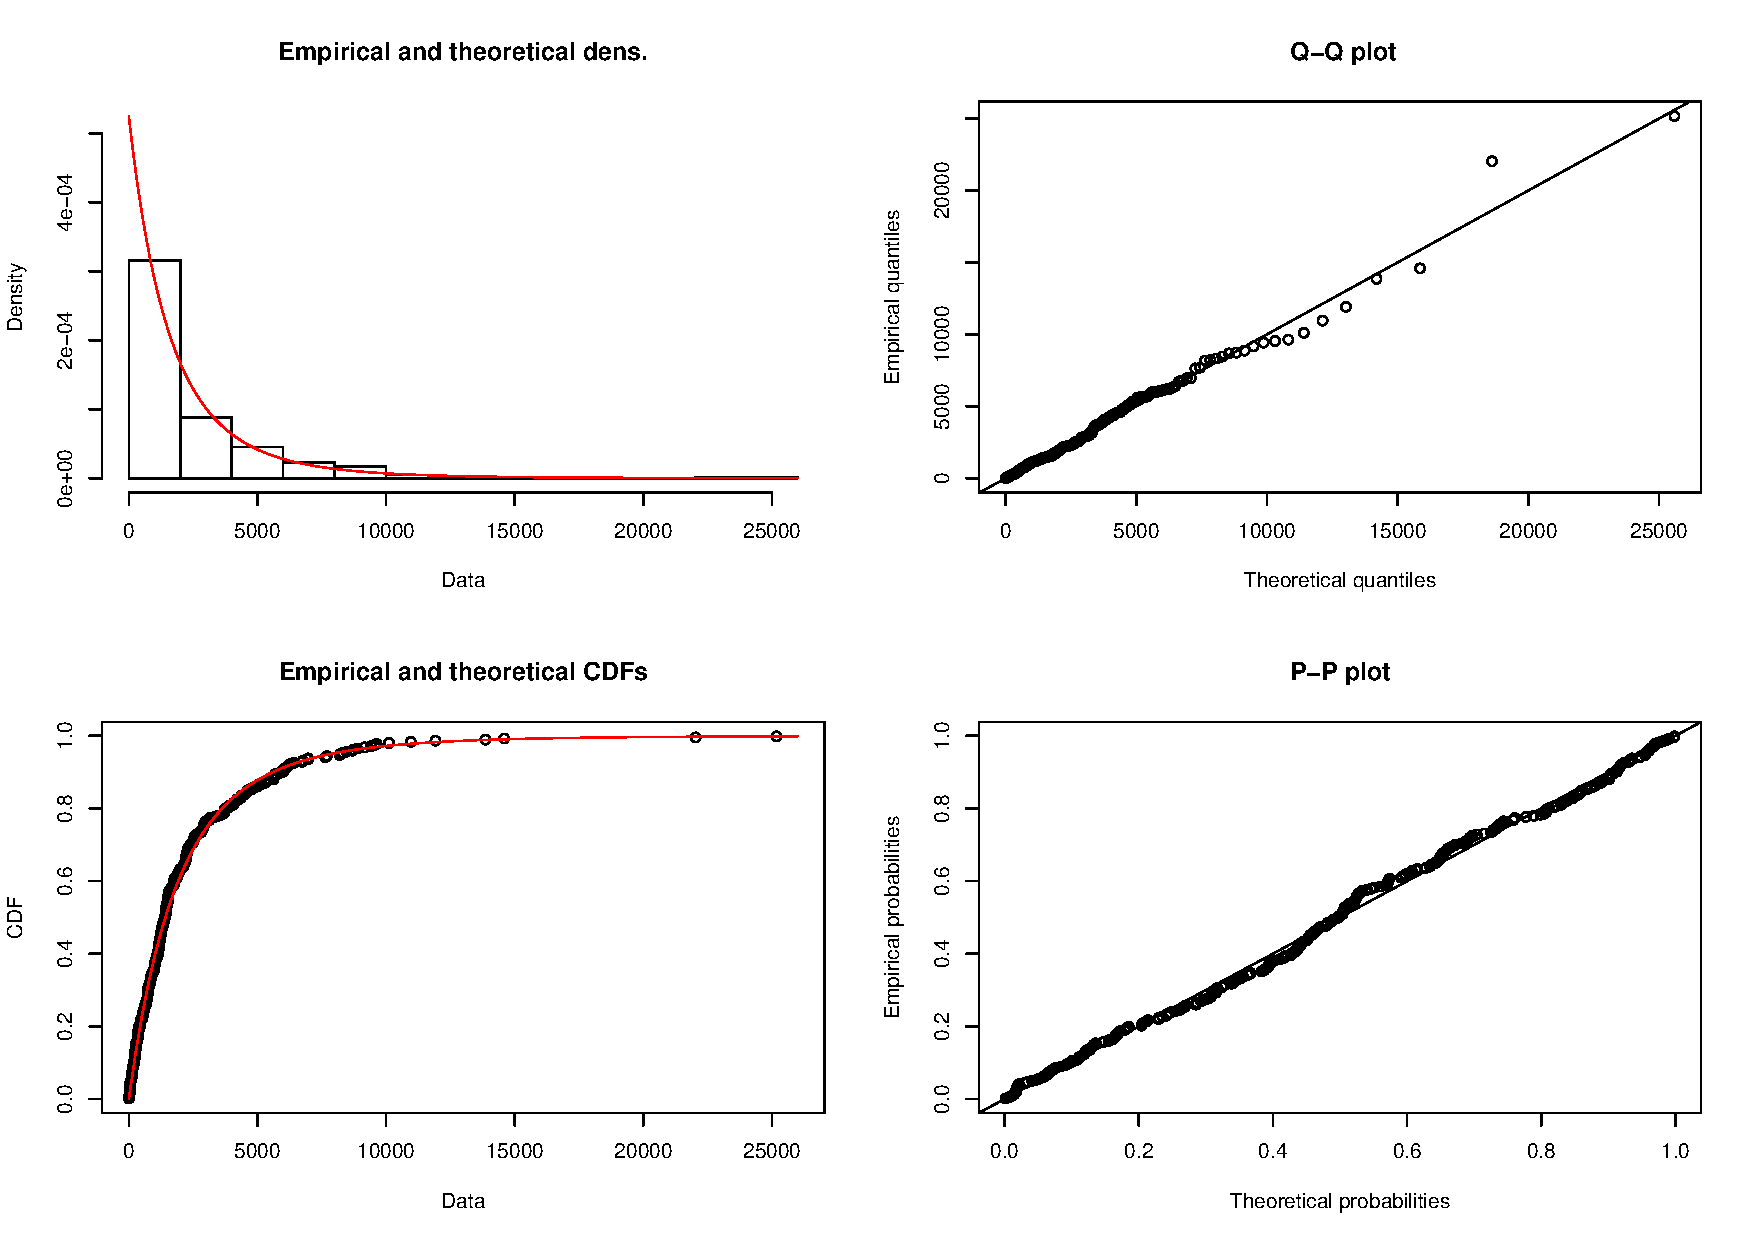
\includegraphics[width=18cm, height=10.5cm]{inter_arrival_pareto.pdf} 
\caption{Density, CDF, P-P and Q-Q plots for a fitted Pareto Distribution against inter-arrival time data}
\end{center}
\label{fig:outagedistribution}
\end{figure*}

Table 3 shows a summary of the seven distributions fitted against the observed inter-arrival time data. Each distribution is listed along with its corresponding Anderson Darling test statistic and p-value. Fig 1 shows four Goodness-of-fit plots for a fitted Pareto distribution: Density, Cumulative Distribution Function (CDF) , Probability (P-P) \cite{gibbons2011nonparametric}  and Quantile (Q-Q) \cite{wilk1968probability}.  


To answer the question of which probability distribution is the most appropriate fit to model the inter-arrival times of Cloud outages, seven continuous distributions were fitted against the data set. To test the goodness of fit an Anderson-Darling (AD) Goodness of fit test was conducted against each probability distribution. 

% Added a clarification around why p-values of < 0.05 are less than desirable.
Our hypotheses question asks: Does the data set follow a specified distribution? We then use a corresponding p-value to test if the data set comes from a chosen distribution. If the p-value is less than 0.05 we can reject the hypothesis (i.e. our data set is unlikely to follow a specific distribution). If the p-value is greater than 0.05 we can accept our hypothesis (i.e. our data is likely to follow a specific distribution). 


With the exception of Pareto and loglogistic distribution, all others were a poor fit indicated by the low p value and the very large AD test statistic. Pareto was found to be the best fit with an AD test statistic of 0.95 and a p-value of 0.38. It is worth noting that as the AD test statistic becomes large the corresponding p-value remains fixed, which explains why the four worst fitting distributions have identical p-values.

Fig 1 graphically illustrates the how well the Pareto distribution fits our dataset. The Q-Q plot shows the majority of data fits the distribution model line, with the exception of a number of large quantiles residing outside the model line. Additionally the P-P and CDF plot also indicates that our data set is a good fit for Pareto with the majority of points positioned along the model line / curve. By and large all points reside on the model line with the exception of the probability values between 0.37 and 0.57. However this observation does not undermine the assumption that the Pareto distribution is a reasonable fit for our data set. 

\subsection{Service time distribution}

\begin {table}
\caption {Service time distributions :  Goodness of fit summary} 
\begin{center}
\begin{tabular}{p{2.1cm} |  p{3.1cm} | p{1.3cm}} \hline \bf{Distribution} & \bf{AD Test Statistic} & \bf{p-value}
\\ \hline lognormal & 0.34 & 0.90
\\ loglogistic & 0.74 & 0.53
\\ Pareto & 1.60 & 0.15 
\\ weibull  & 6.82 & 4.00e-04 
\\ gamma & 272.44 & 1.83e-06	
\\ exponential & Infinity & 1.83e-06
\\ logistic & Infinity  & 1.83e-06	
\\ \hline
\end{tabular}
\end{center}
\end{table}

\begin{figure*}[]
\begin{center}
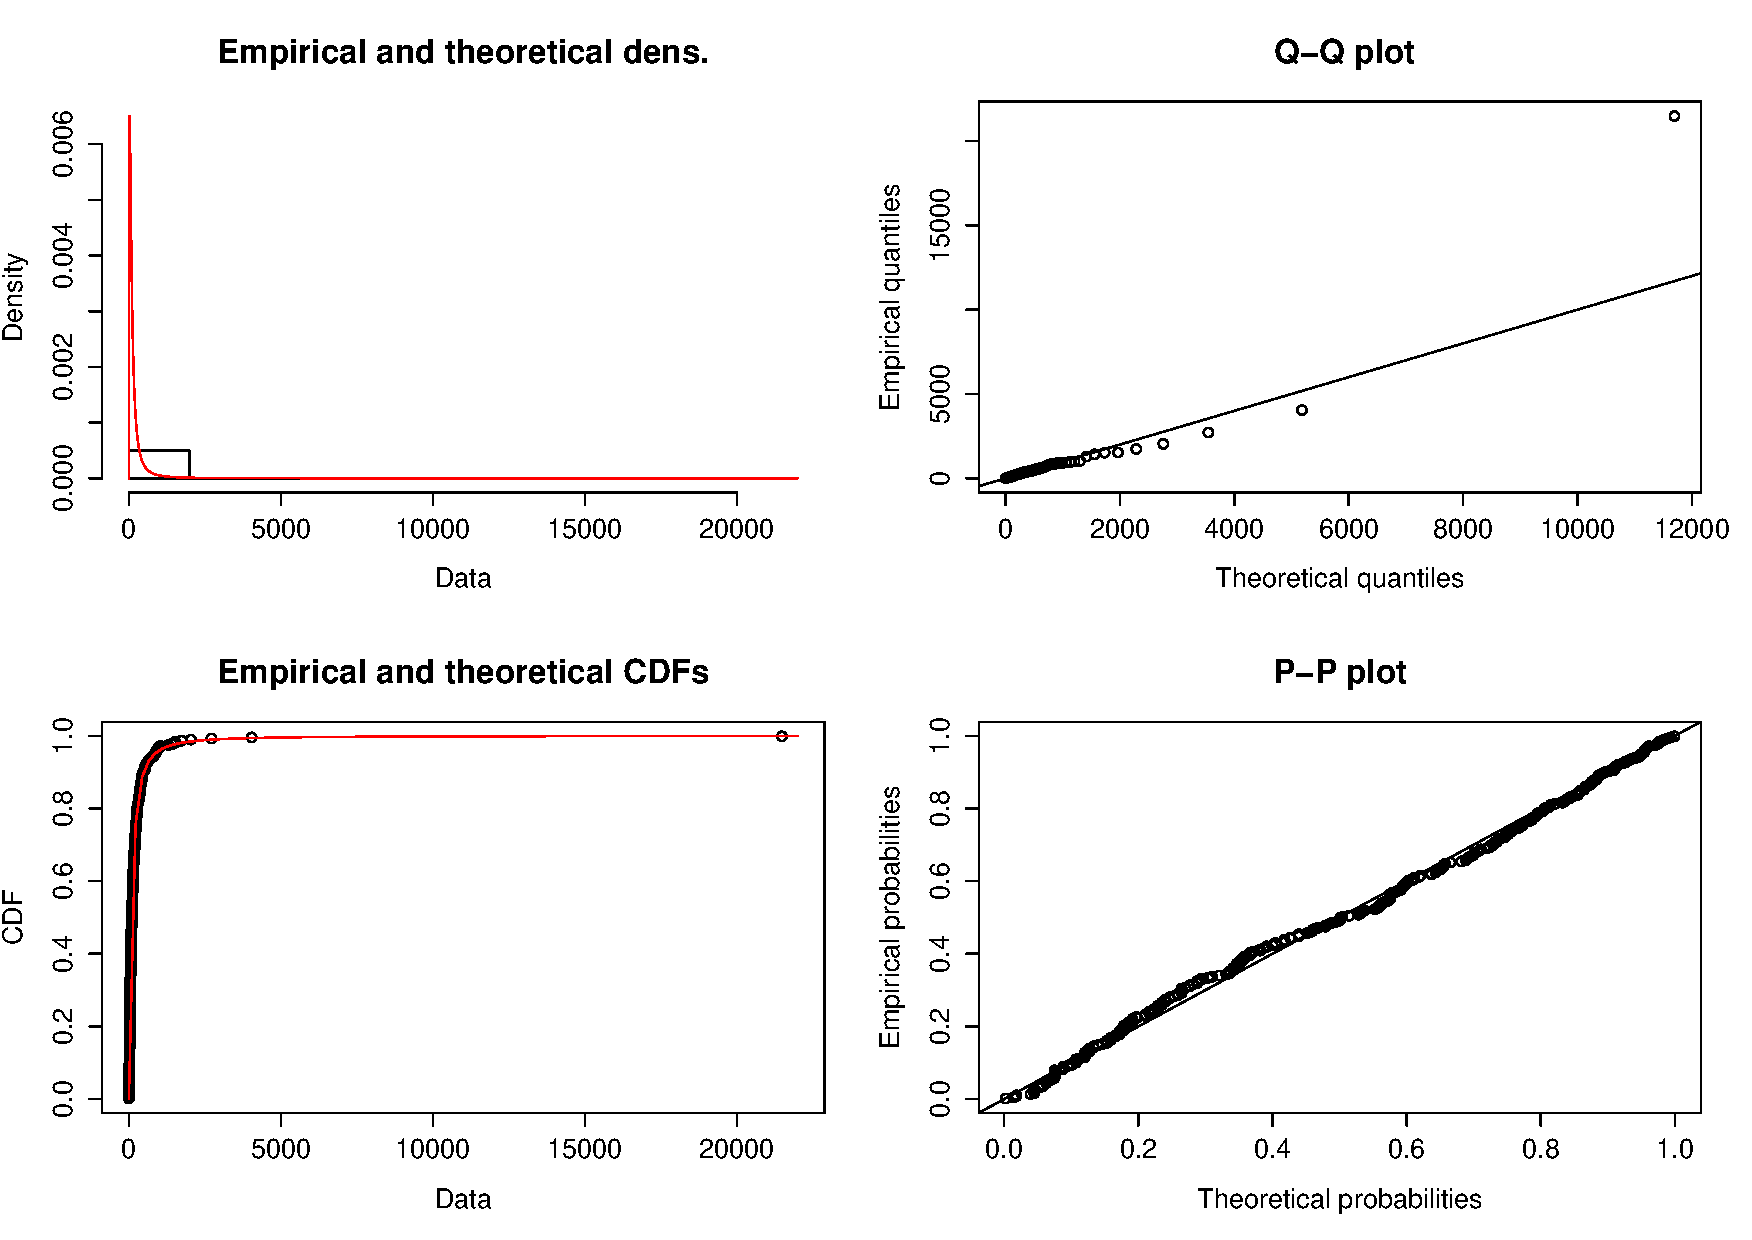
\includegraphics[width=18cm, height=10.5cm]{service_lognormal.pdf} 
\caption{Density, CDF, P-P and Q-Q plots for a fitted lognormal Distribution against service time data}
\end{center}
\label{fig:outagedistribution}
\end{figure*}


Table 4 shows a summary of the seven distributions fitted against the observed service time data. Each distribution is listed along with its corresponding Anderson Darling test statistic and p-value. Fig 2 shows four Goodness-of-fit plots for a fitted lognormal distribution: Density, (CDF), (P-P)  and (Q-Q).  

% Added a clarification around why p-values of < 0.05 are less than desirable.
For the second research question: What probability distribution is an appropriate fit for the observed service times of Cloud outage events, again seven continuous distributions were fitted against the data set. Using the same method for inter-arrival times, an AD Goodness of fit test statistic and p value was computed for each distribution. We also pose the same hypothesis question: Does the data set follow a specified distribution?

Both loglogistic and Pareto scored well, however lognormal was found to be the best fitting with an AD test statistic of 0.34 and a p-value of 0.90. All other distributions had a p-value of \textless 0.05. Once again we can see that as the AD test statistic becomes large the corresponding p-values become fixed around a value of 1.83e-06.

The plots contained in Fig 2 show how the lognormal distribution is a good fit to our dataset. For the Q-Q plot the majority of values fit the distribution line. That said there are a very small number of values with stray from the line, with one obvious extreme value. By and large the fit is very good. Additionally for the P-P plot the values from our dataset either reside on or very close to the line which illustrates the quality of fit.


\subsection{Outage event modelling framework}

\begin {table}[]
\caption {Summary of results from queue modelling experiments and observed overlapping outage events} 
\begin{center}
\begin{tabular}{l | l | l} \bf{Model Type} & \bf {\% Busy} & \bf {\% Free}
\\ \hline Observed Data & 7.9 &  92.1 
\\  Simulation (G/G/1) & 5.7 &  94.3 
\\  Simulation (M/M/1) & 3.0  &  97.0 
\\ \hline 
 \end{tabular}
\end{center}
\end{table}

Now that we have shown the results of distribution fitting, we shall now use these distributions to test our special case of our G/G/1 queue model. For the Pareto distribution our rate and shape parameters were computed to be 4.94 and 9404.06 respectively. Our lognormal service distribution had a computed location and scale parameter of 4.58 and 1.30 respectively.

Table 5 shows a summary of the queue model experiments conducted as well as details of the observed outage data over an eighteen month period. The model type defines whether observed data or a simulation was conducted. The type of simulation is also included. The \% Busy and \% Free columns relate to the number of overlapping events in the queue. Specifically, we counted the number of times an outage event (either observed or simulated) entered the queue system while an existing outage was currently being serviced. This value is presented as an overall percentage. 

As we can see from Table 5, for the observed data the queue was free approximately 92\% (i.e. either 0 or 1 outage was being served) and approximately 8\% of the time the queue was busy (i.e. while an outage was being served another outage event arrived). Comparing the results of both simulations: the G/G/1 simulation compared favourability with the observed results with approximately 94\% and 6\% free and busy time. However the M/M/1 simulation compared less well with 97\% and 3\% free and busy time. Clearly the G/G/1 model gives a better prediction then the M/M/1 model. However the model is still a little optimistic in terms of its forecasting of busy and free times.

% Moved this section 4th as it maps to the fourth research question
\subsection{Correlation between inter-arrival and service times}

\begin{figure*}[]
\begin{center}
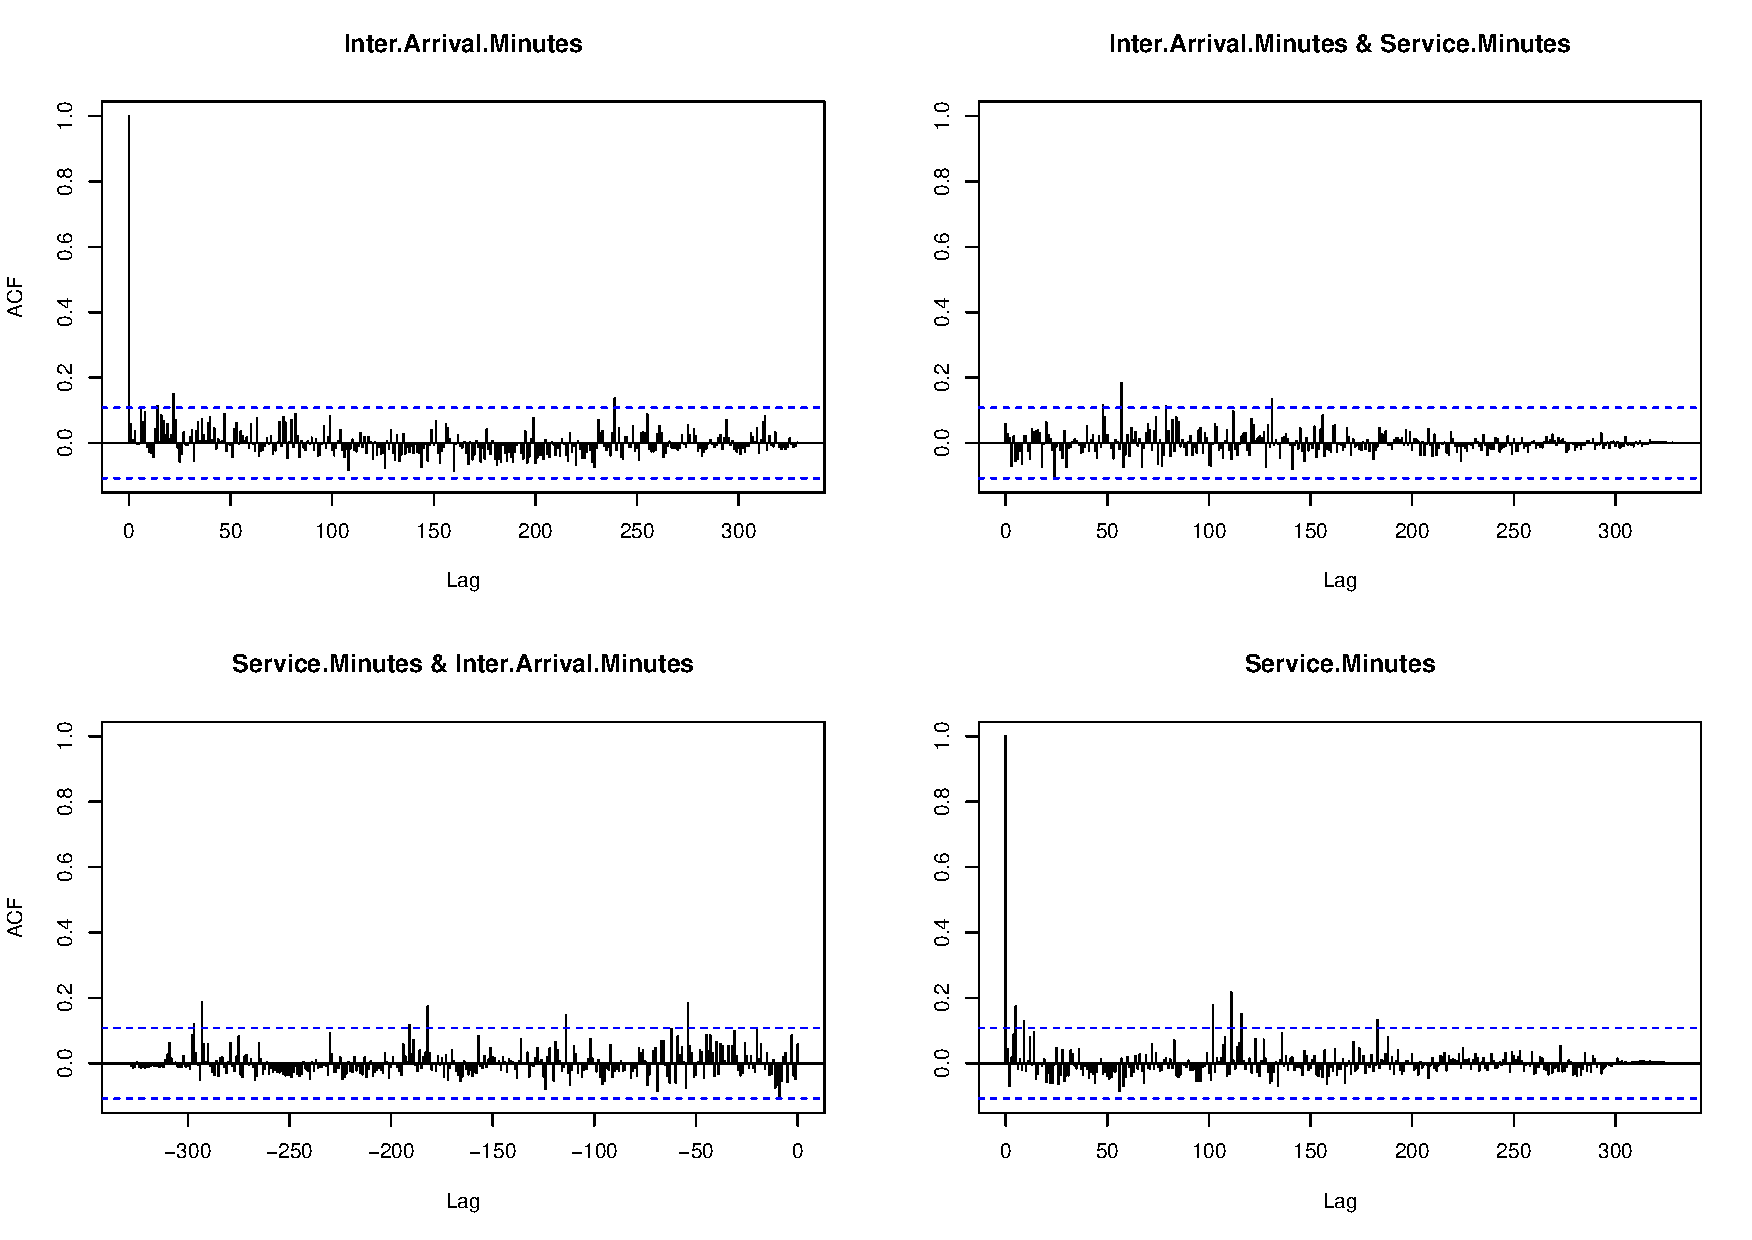
\includegraphics[width=18cm, height=10.5cm]{acf_graph.pdf} 
\caption{Autocorrelation plots for inter-Arrival and service times}
\end{center}
\label{fig:acfgraphs}
\end{figure*}

Figure 3 shows the results of the autocorrelation test between the sequences of inter-arrival and service times. Starting with the inter-arrival times we can see that the lags at positions 0, 25 and 240 respectively cross the confidence interval. With only three values passing the confidence line (and the lag at position 0 being expected), clearly there is little evidence of a seasonality in the values of inter-arrival times. For service times we observed a number of lags outside the confidence interval at positions 0 --10, 100 --120 and 160. While the correlation at lag 0 is expected, there is weak evidence of seasonality for lower and middle values of service times. Finally looking at the graphs of both inter-arrival and service times, we can see two lags at approximately positions 53 and 140 passing the confidence line. This suggests there is weak evidence of association between the two variables.

In addition to looking at the autocorrelation plots, we also performed tests on corresponding pairs of inter-arrival times and services times to determine their relationship. Both Pearson and Spearman tests of correlation were executed. R\textsuperscript{2} values were computed as 0.06 (Pearson) and 0.06 (Spearman). These results indicate there is a minute positive correlation between inter-arrival and service times.

Finally a we ran a linear regression test using inter-arrival times as the dependent variable and service times as the independent variable. Our hypothesis states: There is no association between inter-arrival and service times. A p-value of 0.297 was computed. We can conclude there is weak evidence against our hypothesis. In other words there is little evidence to suggest that inter-arrival and service times are correlated. 

\subsection{Assessment for no association and linkage between overlapping outage events}

Analysis of the inter-arrival times between each of the 331 outages, was conducted to determine how many outage events overlapped. In other words if an outage was currently being serviced by a DevOps resource, did a subsequent outage occur and if so where these overlapping events linked. Our analysis found 26 overlapping outage events. We inspected each outage report to determine if there was a link between these outages and outages already in the queue. As part of this study we looked at the component affected and the root cause to determine whether a link between events was present. 

We found evidence of a link (i.e a common failure pattern) between 7 overlapping outages. It is worth noting that in 4 cases a temporal network outage was the root cause. In 5 cases the E-mail component was the component affected. While no formal regression analysis was conducted, we can conjecture that there is a correlation between Network failures and the E-mail component. Table 6 contains additional analysis of this work.

\begin {table*}[]
\caption {Summary details of overlapping outages with analysis of component area, root cause and linkage assessment} 
\begin{flushleft}
\begin{tabular}{l | l | l | p{9cm} l} \bf{Outage} \# & \bf{Component} & \bf{Root Cause} & \bf{Outage Details} 
\\ \hline  1 & E-mail &  Network & Cascade network failures were observed in the email component.  A second network failure was observed due to latency caused by the first network failure. Assessment: Outages linked.
\\ \hline 2 & E-mail  & Network/Configuration & A network bottleneck was observed. A configuration change was made to alleviate the bottleneck, this change caused additional bottlenecks. Assessment: Outages linked.
\\ \hline 3 & E-mail  & Concurrency &  A failover operation failed to work correctly which caused an outage, while the system was in a failed state, crash log information was not output correctly. Assessment: Outages linked.
\\ \hline 4 & Social & High Availability & A number of nodes in the social component failed due to a server crash. While these nodes were down, extra load was added to the available nodes in the cluster which caused a subsequent outage. Assessment: Outages linked.
\\ \hline 5 & E-mail & Network & A temporal network outage occurred in the E-Mail system. Most of the nodes failed gracefully and returned to normal operations, however a number nodes did not fail gracefully which caused a secondary outage. Assessment: Outages linked.
\\ \hline 6 & E-mail & Configuration & A service on the E-mail system failed due to contention. A config change was made to remediate. The config change caused additional contention further along the service stack. Assessment: Outages linked.
\\ \hline 7 & Collaboration & Network & A temporal network outage occurred in the collaboration component, which caused all nodes to fail gracefully, almost all nodes returned to normal when the network was restored. A number of nodes however were in a hung state (from the initial outage) which caused a secondary outage. Assessment: Outages linked.
\\ \hline 
 \end{tabular}
\end{flushleft}
\end{table*}

Table 7 shows a 2 by 2 contingency table which contains counts of overlapping, non-overlapping, linked and non-linked outage evetns. Fishers exact test was carried out on the table data. Our null hypothesis states there is no association between overlapping and linked outages. A p-value of \textless 0.001 was calculated. Given the low p-value we can reject the null hypothesis. In other words, based on our observations there is evidence to suggest that overlapping outages are linked to a common failure event.

\begin {table}
\caption {Test for no association between overlapping and linked outages using Fisher's exact test} 
\begin{center}
\begin{tabular}{p{2.7cm} |  p{1.1cm} | p{2cm}} \hline \bf{Outage type} & \bf{Linked}  & \bf{Non-linked}
\\ \hline Non-Overlapping  & 0 & 305
\\ Overlapping & 7 & 19
\\ \hline
\end{tabular}
\end{center}
\end{table}

\section{Discussion}

Section 4 presented the results of distribution fitting, queue modelling and test for no association between overlapping outage events. The following section provides deeper analysis and discussion of these results. In each section references will be made to each research question asked in section 3. 

Prior to a detailed discussion of our results, we summarise the results along with each corresponding research question. Table 8 provides this summary

\begin {table*}[]
\caption {Summary of research questions and results} 
\begin{flushleft}
\begin{tabular}{l p{5cm} | l | p{5cm} l} \bf{Research Question} \# & \bf{Results} & \bf{Literature} 
\\ \hline 1. How are the inter-arrival times of Cloud outage events distributed? & E-mail & Cascade 
\\ \hline 2. How are the service times of Cloud outage events distributed? & E-mail  & A network 
\\ \hline 3. How can an effective queuing model be built to simulate outage event traffic? & E-mail  &  A failover 
\\ \hline 4. How are inter-arrival and service times correlated? & Social & A number
\\ \hline 5. Are overlapping outage events related or can we treat each event as independent? & E-mail & A temporal 
\\ \hline 
 \end{tabular}
\end{flushleft}
\end{table*}


\subsection{Inter-arrival time distribution}

The results section has shown that the Pareto distribution is a good fit to model the inter-arrival times of Cloud outage events, which answers our first research question.

The decision to use Pareto as an inter-arrival time distribution is an interesting choice. The Pareto distribution is a power law distribution and has applications in many fields of science. However the field where a Pareto distribution is typically used is in the area of finance. Specifically for modelling income and wealth \cite{arnold2015pareto}. 

The characteristics of our data that make Pareto so attractive is the number of values within a specific range. Inter-arrivals times range from 3 to 1057122 minutes. Using 2500 minutes as an arbitrary point of delineation, 71\% of inter-arrival times were below 2500 minutes, while 29\% were above 2500 minutes. While this split does not conform to the textbook "80-20" rule \cite{chen1993theoretical}, it does illustrate that our data set contains a significantly higher proportion of shorter inter-arrival times than longer ones. Given this specific trait, it is not unsurprising that the Pareto distribution is such a good fit. 

This study has answered our first research question: What distribution can be used to model inter-arrival times of Cloud outage events. DevOps teams can use the shape and scale parameters of their inter-arrival distribution to compute a mean and standard deviation, which can provide an expected time between outage events. Additionally this result can be used to compute the proportion of inter-arrival times above or below a specific duration. These results can be used to aid resource planning. For example, if the expected inter-arrival time is known or if a high proportion of outages is known to occur within a specific duration, duty rosters can be generated to ensure adequate staffing is available when an outage occurs. Finally this results can be used as a component in a wider queue model framework to infer team busy time.

\subsection{Service time distribution}

We have learned from our results that the lognormal distribution is an excellent fit to model the service times of Cloud outage events recorded in our dataset. 

The log-normal distribution is important in the description of natural events. Many natural occurring processes are modelled by the culmination of incremental changes. Such processes include general system usage, vehicle milage per year, count of switch operations and wearout characteristics of machines and systems. This distribution is also versatile in that depending on the location and scale parameters a number of different distribution shapes can be accommodated. 

This result adds to the wealth of existing studies which support the notion that service times for repairable systems can be modelled using a lognormal distribution. We noted previously the work done by Kleyner and O'Connor \cite{o2011practical}. However a number of additional recent studies have observed similar results in their studies of repairable systems such as Apostolakis et al  \cite{apostolakis1980synthesis}, Ananda and Malwane \cite{ananda2003confidence} and Ananda et al \cite{ananda2004steady}. 

This study has answered our second research question: What distribution can be used to model service times of Cloud outage events. DevOps teams can employ the location and scale parameters of their service distribution to compute a mean and standard deviation, which can provide an expected duration service time. With the service times known teams can create schedule plans to determine expected engagement times. Finally this result can be used in conjunction with the result from the previous section to model the idle and busy times of a team as part of a queue modelling exercise.


\subsection{Outage event modelling framework}

We asked the question: How can an effective queuing model be built to simulate outage event traffic? The result from our experiment model shows that a model can be built which is provides a good level of precision compared to observed data.

Table 5 provides a summary of the \% busy and free time for our observed data and for two sets of simulations: G/G/1 and M/M/1 queues. It is unsurprising that M/M/1 lacks precision. There are two factors to consider here. First that neither the inter-arrival nor service distributions could be adequately modelled using an exponential distribution. We recall from Tables 2 and 3 the AD test statistic for the exponential distribution was infinite. For the purposes of the simulation we used the computed means from the Pareto and lognormal distributions. Second the M/M/1 queue assumes that the arrival times between events are independent. We have shown that a small proportion (2\%) of overlapping outage events are linked. These two factors make the M/M/1 queue unsuitable for queue simulation based on the observed data.

Conversely the G/G/1 provided a greater degree of precision than the M/M/1 queue. This is due to the fact that the two distributions selected were a good fit against the observed data compared to the exponential distribution. There is still a minor lack of fidelity between our G/G/1 simulation and our observed data. We can surmise that while the goodness-of-fit for the service time distribution 
was excellent (p-value = 0.90), the goodness-of-fit for the inter-arrival time distribution was very good (p-value = 0.72). Moreover there is the question of independence between arrivals. We must conclude that with a small number of dependent outages coupled with the less than exact fit of the inter-arrival distribution may skew the precision of our simulation. We discuss improvements to this model in future work.

Now let us look at the practical application of such a simulation model. The core of idea of this paper is to produce a model which is effective in simulating the arrival of Cloud events. We have previously mentioned the challenges that both micros teams and SME's have when working in the area of Cloud computing. One of the key challenges is the deployment of resources, and how one can position these resources where they are most needed. Let us consider the following scenario as an example of our simulation framework. 

Table 9 shows the output from a G/G/1 simulation using the parameters from our data set. There are two columns: Time (Measured in minutes) and Queue length. Let assume that  we have uptime from 12:00 1st of January. Looking at the output below we can see that we will need one resource to service the first  thirteen outage events. These thirteen outages will arrive and be serviced in sixteen days. Looking at the fourteenth outage event we can see this event will arrive at approximately 11:18 on the 16th of January. DevOps Management have a good indication that two DevOps resources will be required at this time.  One to service the thirteenth outage and a second resource to service the overlapping fourteenth outage. DevOps management can also infer that both resources will be required for only for a short duration. In this case eight minutes approximately. Thereafter one resource will be needed to debug and remediate subsequent outage events.

Another application of the queue simulation model is to assess staffing requirements over a calendar year. By knowing the duration of a year in minutes (525600) , we can easily check to see how many events will occur during a calendar year. In a simulation conducted for the purposes of this example we found the queue length was greater than 1 on 28 occasions. 27 times the queue length = 2 and once the queue length = 3. A final application is to look at the queue busy time in a given calendar year. If we add the times the queue is busy (i.e. time difference between the queue length being 1 or more and 0) for outages that occur over the period of a year, we can see that the queue will be busy for approximately 144 days. Clearly these types of what if scenarios are very useful for resource planners.


\begin {table}
\caption {Sample output from an G/G/1 simulation} 
\begin{center}
\begin{tabular}{p{1.8cm} |  p{1.25cm} | p{3.2cm}} \hline \bf{Duration (Minutes)} & \bf{Queue Length}  & \bf{Date \& Time}
\\ \hline 2  & 1 & 2017-01-01 00:02
\\ 142 & 0 & 2017-01-01 02:22
\\ 3744 & 1 & 2017-01-03 14:24 
\\ 3761 & 0 & 2017-01-03 14:41
\\ 5577 & 1 & 2017-01-04 20:57
\\ 5644 & 0 & 2017-01-04 22:04
\\ 11043 & 1 & 2017-01-08 16:03
\\ 11048 & 0 & 2017-01-08 16:08
\\ 14989 & 1 & 2017-01-11 09:49 
\\ 15186 & 0 & 2017-01-11 13:06 
\\ 19566 & 1 & 2017-01-14 14:06
\\ 19605 & 0 & 2017-01-14 14:45
\\ 22249 & 1 &  2017-01-16 10:49
\\ 22278 & 2 & 2017-01-16 11:18
\\ 22286 & 1 & 2017-01-16 11:26
\\ \hline
\end{tabular}
\end{center}
\end{table}


\subsection{Correlation between inter-arrival and service times}

Using a myriad of tests we have answered our fourth research question: How are inter-arrival and service times correlated? Our results show that there is little evidence to suggest a correlation between inter-arrival and service times.

Figure 3 showed graphically how both variables were correlated not only with themselves but each other. Given the low number of lags crossing the confidence interval coupled with the sparse positioning of these lags, there is little evidence to suggest any meaningful correlation. Likewise we saw similar results from both the Pearson, Spearman, and linear regression tests. 

DevOps team can use this result in a number of ways. An ideal goal for a cloud based business is to have as near to 100\% uptime as possible, while ensuring that when an outage does occur, that the time to service such an outage is as short as possible. In other words having very long inter-arrival times between outage events and very short service times is highly desirable. The goal for each requires a separate solution, in the case of long inter-arrival times ensuring that when a system does fail, it fails gracefully without any loss of service. In the case of service times, having an advanced suite of system monitoring solutions coupled with a simple system of rollback to prior code versions and/or configuration changes is key. 

Given the lack of correlation between inter-arrival and service times, DevOps teams can be confident that process changes to reduce service times will not lead to a reduction in inter-arrival times. Moreover with increased reliability brings longer inter-arrival times, this in essence will not lead to longer service times.


\subsection{Assessment for no association and linkage between overlapping outage events}

Our results section has highlighted there there is an association between outage events that overlap and outages which are linked (i.e. cascade failures).

Table 6 provides a good insight into the nature of linked outage events we saw that in five of the seven linked outages that E-mail was a common component. Likewise we observed that network and configuration issues were the root causes in four of the seven outages, this may not be a coincidence. In one other case we saw that in a disaster recovery scenario, server node failover did not work as expected which caused a cascade failure due to high concurrency.

Table 7 highlights that overlapping outages are uncommon with approximately 8\% of all outages recorded over an eighteen month period overlapped. Additionally linked outages are rarer still with only approximately 2\% recorded over the same duration. However as demonstrated by the results of Fisher's test, there is overwhelming evidence to suggest that both events are associated. We can calculate when an overlapping event occurs there is a approximately a 25\% probability that these events are linked. Removal of these types of failures is key to the success of a business and will lead to increased customer satisfaction by increased up time. 

DevOps teams can learn from these results, linked failures cause additional workloads for small teams. From a remediation perspective, DevOps team can work with their software development counterparts to ensure their infrastructure and software are more resistance to temporal network outages. By conducting a series of negative tests teams can determine how gracefully their systems fail under scenarios like temporal network outages. Additionally by setting invalid parameters within a large distributed system can have knock on effects. It it worth pointing out that by introducing a system of managed configuration changes (similar to developer code reviews prior to checkin), can help alleviate the problems encountered with invalid configuration changes.

\section{Conclusion}

One purpose of this research was to examine which probability distributions could be used to best model inter-arrival and service times of outages. By using the best fitting distributions as part of a special case of the G/G/1 queue modelling system, this study demonstrated how this model can be used to determine the busy time of a Cloud outage queue system. Additionally this study examined the correlation between inter-arrival and service times. Furthermore we observed whether overlapping outage events are  linked.

It was found that inter-arrival and service times of Cloud outage events could be reasonably modelled with a Pareto and lognormal distribution respectively. Additionally by using these distributions, a queue model framework could be built to infer the percentage busy time of this queue with a good degree of accuracy. Furthermore we found no evidence of correlation between inter-arrival and service times. Finally our research showed that there is evidence to suggest that overlapping outage events are linked.

The findings of this study support previous work specifically in the field of repair times of maintainable Cloud based software systems. This work provides  more comprehensive analysis of the inter-arrival times of Cloud outage events and how using inter-arrival and service time distributions a useful special case of the G/G/1 can be developed to determine queue busy time. 

However the main application of this research is to DevOps and project planners within an SME or micro team. Both can leverage this framework to build an accurate resource planning model which can both identify skill and personal gaps. Identification and remediation of these gaps will greatly benefit teams in the challenging area of Cloud outage resolution.

By using the simple queue as a starting point, future work is planned to validate the framework in the context of a complex queuing system (i.e. a queue with multiple "servers"). John \cite{john1963single} discusses dependencies between inter-arrival and services times within a queue system as the assumption of independence between the two times are not always valid.

Also of interest is the wear our characteristics of specific software components. Conducting a study of Cloud outages as part of a wider renewal process study we can understand the the mean time to failure of a given component.  With the age (uptime) of a component known, how likely is such a component to fail? Finally how often does a component need to be replaced and what role does hygienic recycling play in system stability?

Future work will also include research into the relationship between inter-arrival and service time durations and how these durations relate to service level agreement impact.

\section{Acknowledgements}

This research did not receive any specific grant from funding agencies in the public, commercial, or not-for-profit sectors.

\section*{References}

\bibliography{journal-bib}

\end{document}